\documentclass{article}
\usepackage{amsfonts}
\usepackage{amsthm}
\usepackage{amssymb}
\usepackage{amsmath}
\usepackage{graphicx}
\usepackage{subcaption}
\usepackage{xcolor}
\usepackage{mathtools}
\usepackage{ wasysym }
\usepackage{enumerate}
\usepackage{verbatim}


\numberwithin{equation}{section}
\newcommand{\new}[2]{
    \vspace{2mm}
    \noindent
    \textbf{
    \underline{#1}}
    \textit{{#2}}
    \
}

\def\<{{\langle}}
\def\>{{\rangle}}

\DeclarePairedDelimiter\bra{\langle}{\rvert}
\DeclarePairedDelimiter\ket{\lvert}{\rangle}
\DeclarePairedDelimiterX\braket[2]{\langle}{\rangle}{#1\,\delimsize\vert\,\mathopen{}#2}


\newcommand{\textOr}{
    {
        \hspace{5mm}
        \textrm{or}
        \hspace{5mm}
    }
}

\newcommand{\textAnd}{
    {
        \hspace{5mm}
        \textrm{and}
        \hspace{5mm}
    }
}


\newcommand{\textWhere}{
    {
        \hspace{5mm}
        \textrm{where}
        \hspace{5mm}
    }
}



\newcommand{\Ixp}[1]{
    {
        e^{i{#1}}
    }
}



\newcommand{\halfFigure}[1]{
\begin{center}
\includegraphics[width = .5\linewidth]{{#1}}
\end{center}
}

\newcommand{\fullFigure}[1]{
\begin{center}
\includegraphics[width = .9\linewidth]{{#1}}
\end{center}
}

\def\twobytwoMat(#1, #2, #3, #4){
    {
        \begin{bmatrix}
            {#1} & {#2}\\
            {#3} & {#4}
        \end{bmatrix}
    }
}

\def\twobyoneMat(#1, #2){
    {
        \begin{bmatrix}
            {#1}\\
            {#2}
        \end{bmatrix}
    }
}

\def\twobytwoDet(#1, #2, #3, #4){
    {
        \begin{vmatrix}
            {#1} & {#2}\\
            {#3} & {#4}
        \end{vmatrix}
    }
}


\newcommand{\deriv}[2]{
\frac {d {#1} } {d {#2}}
}

\newcommand{\pderiv}[2]{
\frac {\partial {#1} } {\partial {#2}}
}


\newcommand{\RR}{\mathbb{R}}
\newcommand{\CC}{\mathbb{C}}
\newcommand{\ZZ}{\mathbb{Z}}
\newcommand{\Zpos}{\mathbb{Z}_{pos}}
\newcommand{\NN}{\mathbb{N}}

\newtheorem{theorem}{Theorem}
\newtheorem{proposition}{Proposition}
\newtheorem{lemma}{Lemma}
\newtheorem{corollary}{Corollary}
\newtheorem{remark}{Remark}
\newtheorem{definition}{Definition}
\newtheorem{example}{Example}
\newtheorem{conjecture}{Conjecture}
\newtheorem{question}{Question}

\newcommand{\ch}{\text{ch}}
\title{PHYS 411T Final Exam}
\author{Daiel Son}

\begin{document}
\maketitle

\section{Minis}

\begin{figure}[htp]
    \centering
    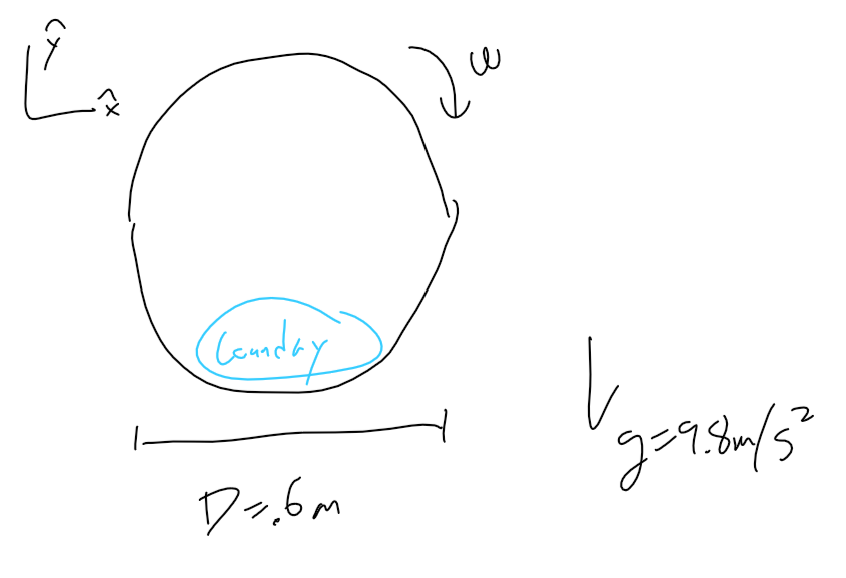
\includegraphics[width=0.8\textwidth]{Q1_Fig.png} % Replace 'figure.jpg' with your image file
    \caption{A simplified laundry basket. }
    \label{fig:example}
\end{figure}

\begin{proof}[Part A]
    Suppose the laundry basket starts rotating at some high 
    angular frequency and slows down gradually. 
    This way, we can ignore the effects of friction 
    and assume that the clothes also move 
    in the same angular velocity as the basket. 
    We wish to find the angular velocity 
    where the laundry loses contact with the surface. 
    This occurs when the gravity exceeds 
    the centrepetal acceleration of the clothes. 
    The threshold angular velocity $\omega$ 
    must satisfy the following. 
\begin{align}
    \vec F_{\rm cent} \ = \ \frac {m v^2} r \ = \ \frac{m (r\omega)^2} r \ = \ mg \\ 
    \boxed{
        \omega \ = \ \sqrt{\frac g r  } \ = \ 5.715 rad/s
    }
\end{align}\footnote{The corresponding period is about $1.1s$ per cycle. }
    
\end{proof}

\begin{proof}[Part B]
    Two objects in space that 
    interact only through Newtonian gravity 
    must orbit one another either in an elliptic orbit or a circular orbit. 
    
\end{proof}

\begin{proof}[Part C] The following is the formula for 
    inertia tensor elements. 
    \begin{align}
        I_{ij} \ = \ \sum_\alpha m_\alpha\left( \delta_{ij}\vec r \cdot \vec r - r_i r_j\right)
    \end{align}
\end{proof}

\begin{proof}[Part D] Here are the Hamilton's equations. 
\begin{align}
    \pderiv{H}{p_i} \ = \ \dot q_i \textAnd
    \pderiv{H}{q_i} \ = \ - \dot p_i
\end{align}
    
\end{proof}

\section{Von Braun's Space Station}

\begin{figure}[htp]
    \centering
    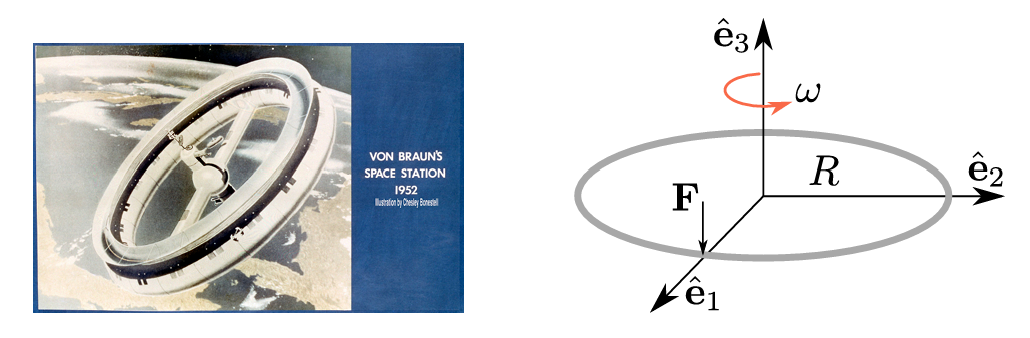
\includegraphics[width=0.8\textwidth]{Q2_fig.png} % Replace 'figure.jpg' with your image file
    \caption{Von Braun's Space Station.}
    \label{fig:example}
\end{figure}

\begin{proof}[Part A]
    Assume the space station to be a ring of radius $R$, 
    and ignore the width and height. 
    We compute the inertia tensor of the space station. 
    First, observe that the off diagonal elements are zero. 
    \begin{align}
        \int xz \ dm \ = \ \int yz \ dm  \ = \ 0
    \end{align}
    These integrals vanish because $z = 0$ around the 
    entirety of the space station. 
    \begin{align}
        \int xy \ dm 
    \end{align}
    This integral vanishes, since every infinesimal 
    chunck of the space station as a corresponding chunk 
    which is symmetric to the $x$-axis. 

    Secondly, compute the following integrals. 
    \begin{align}
        \int z^2 \  dm\ = \ 0 \textAnd  \int y^2 \ dm = \int x^2 \ dm
    \end{align}
    The first integral vanishes by the same argument above, and 
    the latter two integrals agree by symmetry. Evaluate the $x$ integral.
    Denote the linear mass density of the station as 
    $\lambda = M/(2\pi R)$ 
    \begin{align}
        \int x^2 dm \ = \ \int_0^{2\pi} R^2 \cos^2(\theta )\ \lambda R d\theta 
        \ = \ \lambda R^3 \pi \ = \ \frac {M R^2} 2
    \end{align}
    This allows us to compute the diagonal elements of 
    the inertia tensor. 
    \begin{align}
        I_{xx} & = \ 
        \int y^2 \ dm + \int z^2 \ dm \ = \ \frac {MR^2} 2 \\ 
        I_{yy} & = \
        \int x^2 \ dm + \int z^2 \ dm \ = \ \frac {MR^2 } 2\\ 
        I_{zz} & = \  
        \int x^2 \ dm + \int y^2 \ dm \ = \ \frac {MR^2 } 2 + \frac {MR^2 } 2 \ = \ MR^2 
    \end{align}
    Therefore the inertia matrix is 
    \begin{align}
        I \ = \ 
        \begin{bmatrix}
            \frac {MR^2} 2 & 0 & 0 \\ 
            0 & \frac {MR^2} 2 & 0 \\ 
            0 & 0 & MR^2
        \end{bmatrix}. 
    \end{align}
\end{proof}

\begin{proof}[Part B] 
    The magnitude angular velocity vector $\omega$ must satisfy the 
    following. 
    \begin{align}
        \frac {v^2} R & = \ R \omega^2 \ = \ g \\ 
        \omega & = \ \sqrt{\frac g R}
    \end{align}
    Upon inspection $\vec \omega = \omega \hat z$. Also, 
    the angular momentum can be computed as the image of the angular 
    velocity vector under the inertia tensor. 
    \begin{align}
        \vec L \ = \ I \vec \omega \ = \ \omega I_{zz} \hat z \ = \ 
        \sqrt{\frac g R} MR^2 \hat z \ = \ 
        \sqrt{gM^2 R^3}\hat z
    \end{align}
    Here is the answer. 
    \begin{align}
        \boxed{
        (\vec \omega, \vec L) \ = \ 
        \left(
            \sqrt{
                \frac g R
            }\hat z , 
            \sqrt{g M^2 R^3} \hat z
        \right)
        }
    \end{align}
\end{proof}

\begin{proof}[Part C]
    From Euler's equation of torque, we can write 
    out the time evolution of the angular momentum 
    operator as follows. 
    \begin{align}
        \deriv{}{t}\vec L + \vec \omega \times \vec L  \ = \ \vec \tau \ = \ \vec r \times \vec F
    \end{align}
    Assuming that the time $\Delta t$ and the force $F$ is small enough, 
    we can assume that $\vec \omega \times \vec L \approx 0$ since both vectors are 
    approximately parallel to $\hat z$.\footnote{
        Another way to justify this assumption is to 
        ignore the relativistic correction. If 
        the spaceship leaves quickly enough, the motion 
        of the spaceship at the time of departure is 
        approximately the same in both frames. 
    } Therefore, 
    \begin{align}
        \deriv{}{t} \vec L \ = \ R \hat x \times (-z F) \ = \ RF \hat y
    \end{align}
    and the angular momentum changes at a constant rate. After time $\Delta t$, 
    the final angular momentum is 
    \begin{align}
        \vec L_{\Delta t} \ = \ \vec L + \Delta t RF \hat y \ = \ 
        \sqrt{g M^2 R^3} \hat z +  \Delta t RF \hat y
    \end{align}
    \textcolor{blue}{Though the perturbation of the angular momentum is small, $\vec L$ 
    points in a slightly different direction along the $yz$-axis after 
    the spacecraft leaves. }

    It remains to justify that the cross product $\vec \omega \times \vec L$ 
    is negligible. Take some time $t_1 \in (0, \Delta t)$. The angular momentum 
    can be extracted by changing $\Delta t$ to $t_1$, and the angular velocity by taking the 
    inverse image of the inertia tensor. 
    
    \begin{align}
        \vec L_{t_1} & = \ t_1 R F \hat y + \sqrt{g M^2 R^3} \hat z \\ 
        \vec \omega_{t_1} & = \ \frac 1 {MR^2} \left(
            2 t_1 RF \hat y + \sqrt{g M^2 R^3} \hat z
        \right) \\ 
        \vec\omega_{t_1}\times\vec L_{t_1} & = \ t_1 F \sqrt{g R}
    \end{align}
    Under the assumption $\Delta t F \ll 1$, our assumption is justified. 
\end{proof}

\section{Jiggly Pendulum}

\begin{figure}[htp]
    \centering
    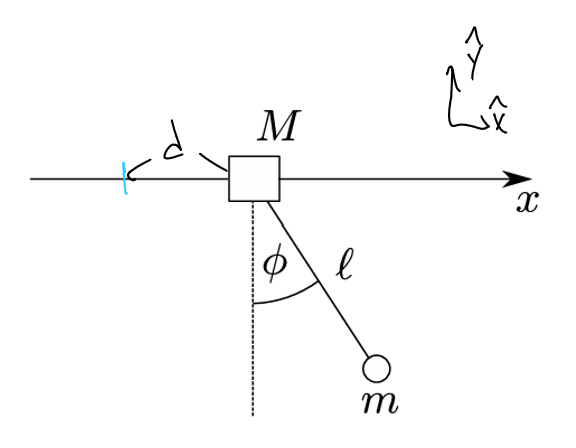
\includegraphics[width=0.8\textwidth]{Q3_fig.png} % Replace 'figure.jpg' with your image file
    \caption{Free body diagram of a Jiggly Pendulum. }
    \label{fig:example}
\end{figure}

\begin{proof} [Part A]
    The crux of constructing the Lagrangian is to find the 
    kinetic energy of the swinging mass. Let $d$ be the displacement 
    of the cart. By vector addition, we obtain the displacement of the 
    swinging mass which we name $\vec r$. 
    \begin{align}
        \vec r \ = \ d \hat x + l \sin(\phi) \hat x - l \cos(\phi) \hat y
    \end{align}
    Take the derivative to retrieve the velocity, and retrieve the 
    squred magnitude. 
    \begin{align}
        \deriv{}{t} \vec r & = \ \dot d \hat x + l \dot \phi \cos(\phi) \hat x + l \dot \phi \sin(\phi) \hat y \\ 
        \bigg\|\deriv{}{t} \vec r\bigg\|^2  & = \ (\dot d)^2 + (l \dot \phi)^2 + 2l \dot d \dot \phi \cos(\phi)
    \end{align}
    From here, simple algebra yields the kinetic energy of the 
    system, which is the sum of the kinetic energy of the swinging 
    mass and the cart. The potential energy comes from gravitational 
    potential of the mass. Let $M, m$ be the mass of the cart and the 
    swinging mass respectively. 

    \begin{align}
        T & = \ T_{\rm cart} + T_{\rm mass} \ = \ \frac 1 2 (M (\dot d )^2 + m (\dot r)^2) \\ 
        & = \ 
        \frac {M + m} 2 (\dot d)^2  + \frac m 2 (l \dot \phi)^2 + 
        m (\dot d) (\dot \phi) l \cos(\phi)  \\ 
        U & = \ -mgl \cos(\phi) \\ 
        \mathcal L & = \ T - U \ = \ \boxed{\frac {M + m} 2 (\dot d)^2  + \frac m 2 (l \dot \phi)^2 + 
        m (\dot d) (\dot \phi) l \cos(\phi) + mgl \cos(\phi)}
    \end{align}
\end{proof}

\begin{proof}[Part B] The Euler-Lagrange equation provides two identities 
    that describes the motion. 
    \begin{align}
        \pderiv{\mathcal L}{ d} \ = \ \deriv{}{t} \pderiv{\mathcal L}{\dot d} \textAnd 
        \pderiv{\mathcal L}{\phi} \ = \ \deriv{}{t} \pderiv{\mathcal L}{\dot \phi}
    \end{align}
    Bash out the algebra to obtain the two equations. 
    \begin{align}
        0 \ =\ (M + m) \ddot d + m \ddot \phi l \cos(\phi) - m (\dot \phi)^2 l \sin(\phi) \\ 
        -2(\dot d) (\dot \phi) l \sin(\phi) - gl\sin(\phi) \ = \ 
        l^2 \ddot \phi + (\ddot d) l \cos(\phi) - (\dot d) (\dot \phi) l \sin(\phi)
    \end{align}
    In fact, the Lagrangian does not have an explicit dependence on 
    the displacement $d$. Therefore, the general momentum in 
    the $d$ direction is invariant.
    \begin{align}
        \deriv{}{t} \left(
            (M + m) \dot d + m (\dot \phi) l \cos(\phi)
        \right) \ = \ 0
    \end{align}
\end{proof}

\begin{proof}
    [Part C] Lets simplify the equations from part B. In the small 
    angle limit, all higher order terms other than the constant and 
    linear terms can be ignored. Moreover, $\sin(\phi) = \phi$ and $\cos(\phi) = 1$. 
    We obtain the follwing. 
    \begin{align}
        0 \ = \ (M + m) \ddot d + m l \ddot \phi \\ 
        -gl \phi \ = \ l^2 \ddot \phi +  l \ddot d 
    \end{align}
    Convert $\ddot d$ to $\ddot \phi$ and plug in to the second equation. 
    \begin{align}
        \frac M {M + m} \ddot \phi \ = \ - \frac g l \phi \\ 
        \ddot\phi \ = \ - \frac {g (M + m)}{lM} \phi
    \end{align}
    Thus, the frequency is 
    \begin{align}
        \omega \ = \ \sqrt{\frac {g (M + m)}{lM}}
    \end{align}
    Clearly, if $M \gg m$, then $\frac {M + m} M = 1$ and we obtain 
    the frequency 
    \begin{align}
        \omega_{M\gg m} \ = \ \sqrt{\frac g l}
    \end{align}
    which is the frequency of a regular fixed pendulum. 
\end{proof}

\begin{proof}[Part D]
    The general solution for $\phi(t), d(t)$ is described as follows. 
    \begin{align}
        \phi(t) & = \ \phi_0 \cos(\omega t + a) \\ 
        d(t) & = \ - \frac {ml}{M + m} \phi_0 \cos(\omega t + a)
    \end{align}
    We wish to draw a state space diagram for $\phi(t)$. Assume the 
    initial condition $\phi(0) = \phi_0$ and $\dot \phi(0) = 0$. Then, 
    the angular displacement and velocity is
    \begin{align}
        \phi(t) & = \ \phi_0 \cos(\omega t) \\ 
        \dot \phi(t) & = \ -\omega\phi_0 \sin(\omega t)
    \end{align}
    Below is a sketch of the solution in time. Note that the angular 
    displacement of the mass has an opposite sign as the linear displacement of the cart. 
    \begin{figure}[h]
        \centering
        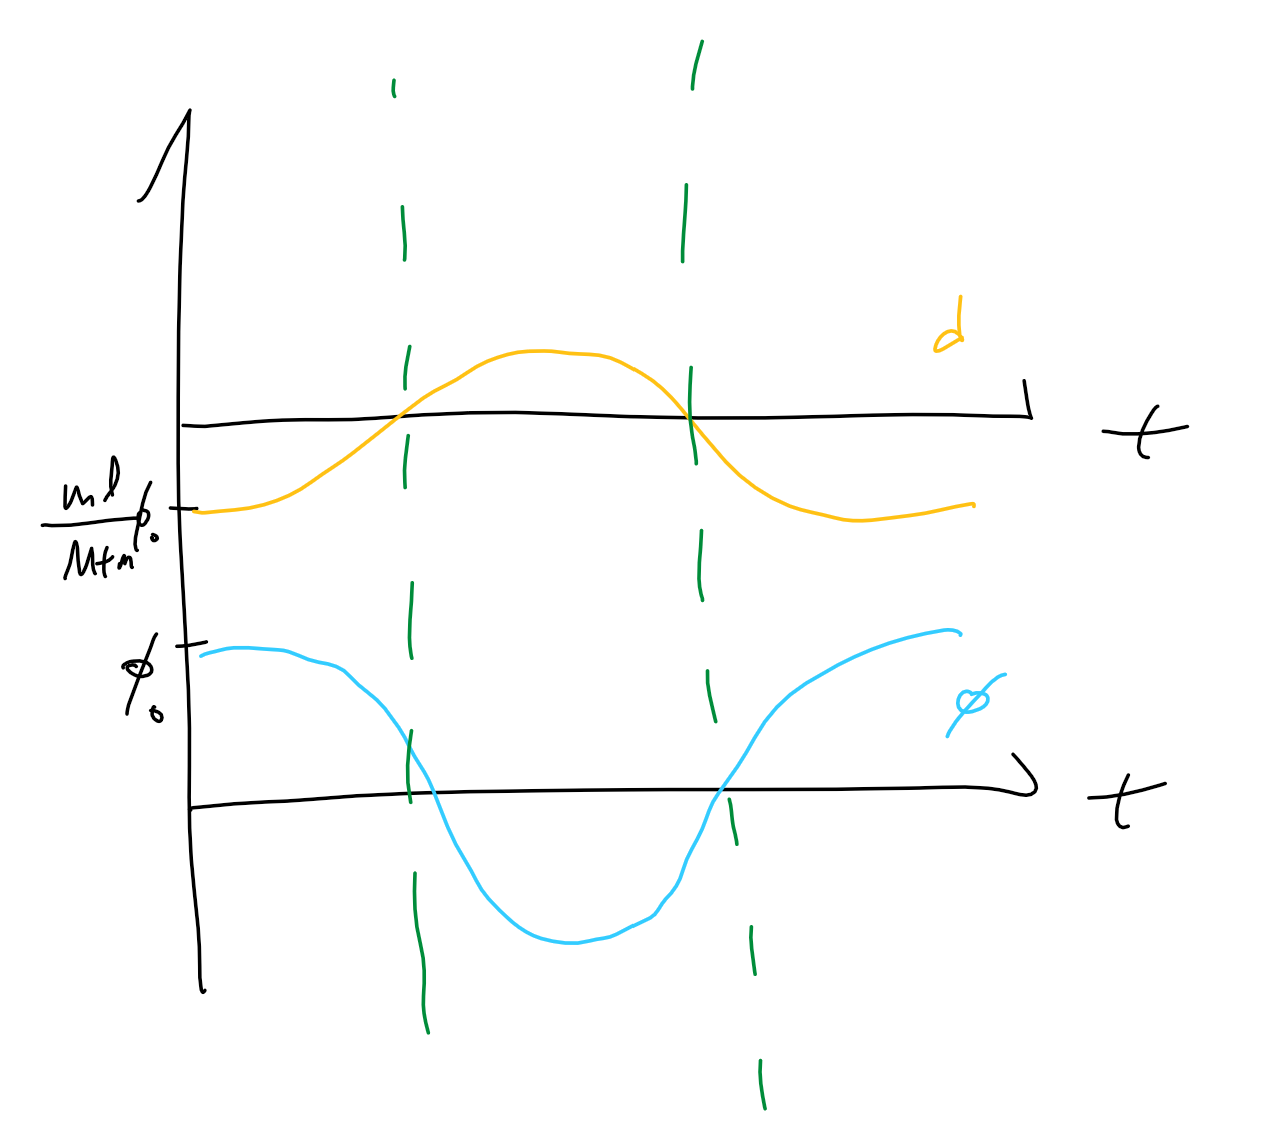
\includegraphics[width=0.3\textwidth]{Q3_statespace.png} % Replace 'figure.jpg' with your image file
        \caption{Time progression of $ d(t), \phi(t)$. }
        \label{fig:example}
    \end{figure}
    
    
\end{proof}

\begin{proof}[Part E]
    The hidden normal mode is the symmetric mode where both the cart 
    and the mass move/swing in the same direction. This is a natural 
    assumption, since we have deduced an antisymmetric mode with a $\pi$ 
    phase shift between $d$ and $\phi$. 
\end{proof}

\section{Rotating Spring Revisited}

\begin{proof}
    [Part A] We compute the Hamiltonian from the Lagrangian. From 
    the sum of genaral velocities and general momentum, subtract the Lagrangian. 
    \begin{align}
        \mathcal H & = \ \sum_i p_i q_i - \mathcal L \ = \ 
        \dot r(m \dot r) + \dot \phi (mr^2 \dot \phi) - 
        \frac 1 2 m (\dot r^2 + r^2 \dot \phi^2) + \frac 1 2 k (r- a)^2 \\
        & = \ \boxed{
        \frac 1 2 m (\dot r^2 + r^2 \dot \phi^2) + \frac 1 2 k (r- a)^2
        } 
    \end{align}
    The generalized momentum is computed by taking the partial derivative 
    of the lagrangian with respect to generalized velocity. \textcolor{blue}{
        Upon inspecting Hamilton's equations, we notice that the Hamiltonian 
        itself and the generalized angular momentum is preserved. 
    }The Lagrangian does not depend on time. Therefore, invoke Beltrami's identity 
    to see that the Hamiltonian is constant. \footnote{Or, one can take the 
    time derivative of the Hamiltonian and invoke the chain rule. Invoking 
    Euler-Lagrange equation on the partials will yield the same result. } Also, the 
    Hamiltonian does not have an explicit $\phi$ dependence. Therefore, 
    \begin{align}
        \pderiv{\mathcal H}{ \phi} \ = \ -\dot p_\phi = 0
    \end{align}
    and $ p_\phi$ is invariant. 
\end{proof}

\begin{proof} [Part B]
    The invariant angular momentum is 
    \begin{align}
        p_\phi \ = \ m r^2 \dot \phi. 
    \end{align}
    Let $r_0, \omega$ be the equilibrium radius and angular velocity. 
    Then, 
    \begin{align}
        p_\phi \ = \ m r_0^2 \omega 
    \end{align}
    which yields 
    \begin{align}
        (r_0, \omega) \ = \ \left(
            \sqrt{\frac{p_\phi}{m \omega}}, \frac{p_\phi}{mr_0^2}
        \right)
    \end{align}
\end{proof}

\begin{proof} [Part C]
    \textit{As long as we get the results, it is better to do less work. }
    Apply Lagrange's equation w.r.t $r$. 
    \begin{align}
        \pderiv{\mathcal L}{r} \ = \ \deriv{}{t} \pderiv{\mathcal L}{\dot r} 
        \textOr 
        m r (\dot \phi)^2 - k (r - a) \ = \ \deriv{}{t} (m \dot r)
    \end{align}
    The RHS of the equation vanishes, assuming circular motion. Solve for $\dot \phi$. 
    \begin{align}
        \dot \phi \ = \ \sqrt{
            \frac k m \frac {r - a} r
        }
    \end{align}
    Since $a$ is a positive length, the fraction $(r-a)/r$ is strictly 
    less that $1$ and asymptotes to $1$ as $r \rightarrow \infty$. 
    Thus, the maximum value of $\dot \phi$ is attained when $a/r \rightarrow 0$. 
    Finally, 
    \begin{align}
        \dot \phi_{\rm max} \ = \ \sqrt{\frac k m} 
    \end{align}
    as desired. 
\end{proof}

\section{Wobble of the Earth}
\begin{proof}[Part A] 
    Assuming the inner core has three times the density of the 
    outward shell, we wish to find the density of the shell, namely $\rho$. 
    The mass can be computed by adding an oblate spheroid with dimensions 
    $(a, b, c)$, density $\rho$ with a sphere of radius $c/2$, density $2\rho$. 
    Equate the sum of the two masses to the mass of the earth. 
    \begin{align}
        \rho V_{ob} + 2\rho V_{sp} \ = \ M_E \\ 
        \frac {4\pi} 3 \rho \left(
            abc + \frac {2 c^3} 8 
        \right)  \ = \ 
        M_E \\ 
        \rho \ = \ \frac 3 {4\pi}M_E \bigg/ \left(
            a^2 c + c^3/4 
        \right)\ = \ \boxed{ 4416 kg/m^3}
    \end{align}
    \begin{figure}[h]
        \centering
        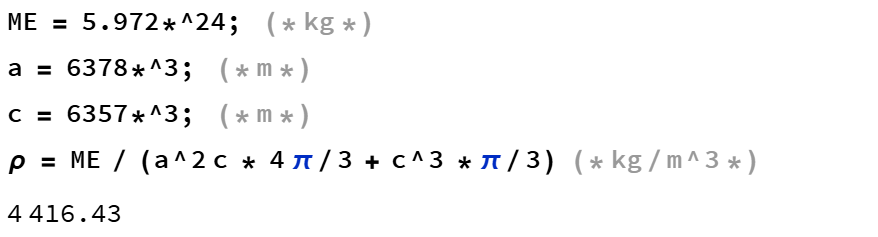
\includegraphics[width=0.8\textwidth]{Q5_a.png} % Replace 'figure.jpg' with your image file
        \label{fig:example}
    \end{figure}
    
\end{proof}
\begin{proof}[Part B]
    The Inertia tensors add up just like masses. Therefore, take the inertia 
    tensor of the oblate spheroid, and add it with the tensor of the sphere. 
    Remember that the core has twice the density as the shell. 

    Remember the formula for the inertia of an oblate spheroid. 
    \begin{align}
        I \ = \ \begin{bmatrix}
            b^2 + a^2 & 0 & 0 \\ 
            0 & a^2 + c^2 & 0 \\ 
            0 & 0 & a^2 + b^2 
        \end{bmatrix} \frac M 5
    \end{align}
    The off diagonal entries of the inertia tensor of earth vanish. 
    Below are the diagonal entries of the inertia tensor of the entire earth. 
    \begin{align}
        (I_{xx}, I_{yy}, I_{zz}) & = \ (8.24\cdot 10^{37}, 8.24\cdot 10^{37}, 8.26\cdot 10^{37}) \\ 
        I_{zz}/I_{xx} & = \ 1.00311
    \end{align}
    so the theoretical inertias match with the experimental inertias 
    up to the first signifigant figure. 

    \begin{figure}[h]
        \centering
        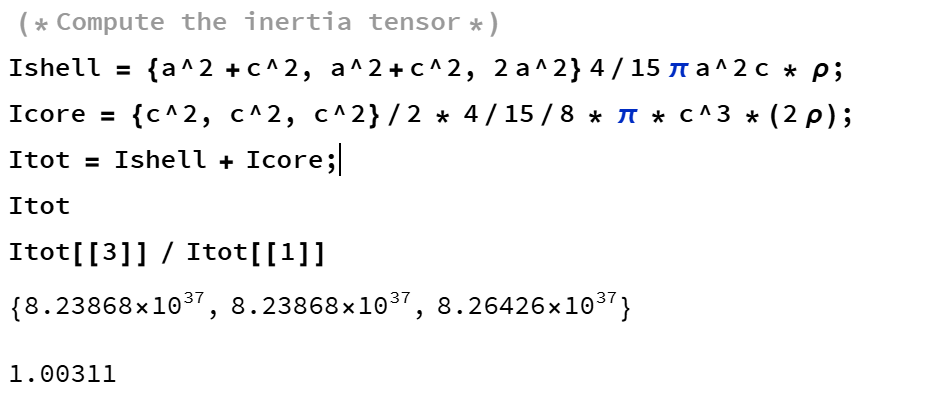
\includegraphics[width=0.8\textwidth]{Q5_b.png} % Replace 'figure.jpg' with your image file
        \label{fig:example}
    \end{figure}
    
\end{proof}

\begin{proof}[Part C]
    Invoke (t10.93) to compute the frequency of the free precession. 
    \begin{align}
        \Omega_b \ = \ \frac{\lambda_1 - \lambda_3}{\lambda_1} \omega_3
    \end{align}
    The angular velocity of the earth points towards the z-axis, and 
    the magnitude can be computed by 
    \begin{align}
        \omega \ = \ \frac{2\pi \ rad}{24\cdot 3600 sec}. 
    \end{align}
    Plug and chug into mathematica. 
    \begin{align}\boxed{
        T = 307.7 \text{days}
    }
    \end{align}
    \begin{figure}[h]
        \centering
        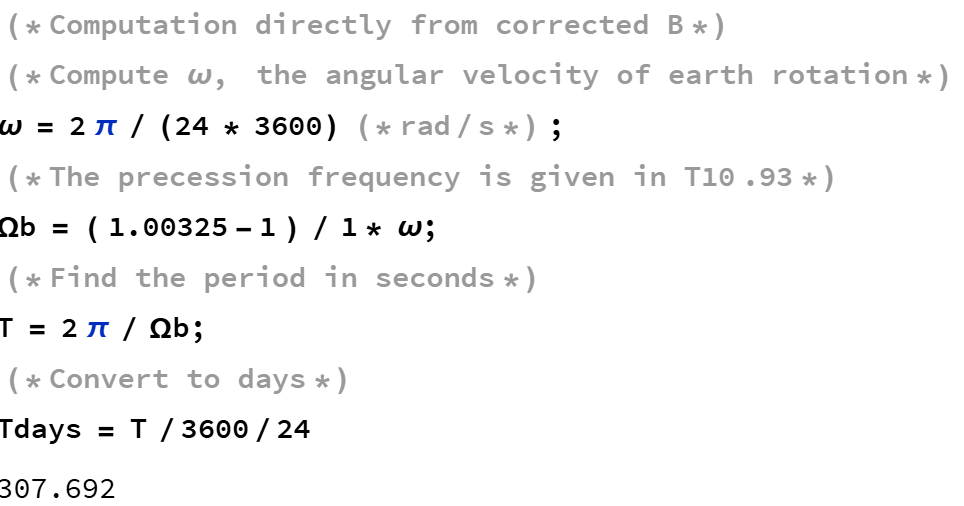
\includegraphics[width=0.8\textwidth]{Q5_c.png} % Replace 'figure.jpg' with your image file
        \label{fig:example}
    \end{figure}
\end{proof}
\footnote{
    Thank you for a wonderful 
    sememster, Professor Jensen and 
    Professor Strauch. I feel more 
    confident about solving problems with 
    where the details of the system are unknown. 
    See you again next sememster, and Merry Christmas!
}

\end{document}